\documentclass[border=3pt,tikz]{standalone}
\usetikzlibrary{arrows}
\usetikzlibrary{positioning}
\usetikzlibrary{calc}
\usetikzlibrary{arrows}
\usetikzlibrary{decorations.pathreplacing}
\begin{document}
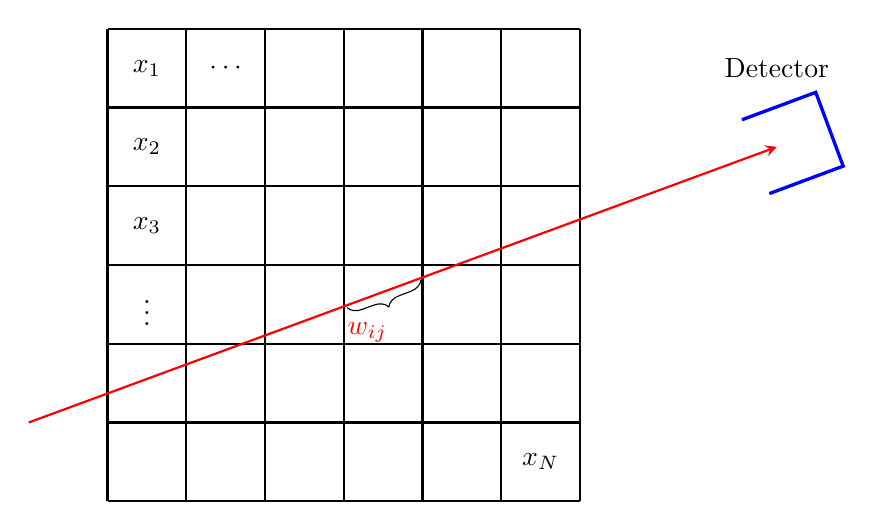
\begin{tikzpicture}
    \draw[step=1.0,black,thick] (-3,-3) grid (3,3);
    \node at (-2.5, 2.5) {$x_{1}$};
    \node at (-2.5, 1.5) {$x_{2}$};
    \node at (-2.5, 0.5) {$x_{3}$};
    \node at (-2.5, -0.5) {$\vdots$};
    \node at (-1.5, 2.5) {$\cdots$};
    \node at (2.5, -2.5) {$x_N$};
    \node at (5.5, 2.5) {Detector};
    \draw[red, thick, -{stealth}] (-4, -2) -- (5.5, 1.5);
    
    \begin{scope}[shift={(5.7,1.55)},rotate=20.4]
    \draw[blue, very thick] (-0.5,-0.5) -- (0.5,-0.5) -- (0.5,0.5) -- (-0.5,0.5); 
    \end{scope}
    
    \begin{scope}[shift={(0.3, 0.2)},rotate=20.4]
    \draw [decorate,decoration={brace,amplitude=5pt,mirror,raise=4ex}]
      (-0.5,0) -- (0.5,0) node[midway,yshift=-3em, red]{$w_{ij}$};
    \end{scope}
    \end{tikzpicture}
\end{document}